 %!TEX TS-program = lualatex
%!TEX encoding = UTF-8 Unicode

\label{key}\documentclass[t]{beamer}

%%%% HANDOUTS For online Uncomment the following four lines for handout
%\documentclass[t,handout]{beamer}  %Use this for handouts.
%\includeonlylecture{student}
%\usepackage{handoutWithNotes}
%\pgfpagesuselayout{3 on 1 with notes}[letterpaper,border shrink=5mm]
%	\setbeamercolor{background canvas}{bg=black!5}


%%% Including only some slides for students.
%%% Uncomment the following line. For the slides,
%%% use the labels shown below the command.

%% For students, use \lecture{student}{student}
%% For mine, use \lecture{instructor}{instructor}


%\usepackage{pgf,pgfpages}
%\pgfpagesuselayout{4 on 1}[letterpaper,border shrink=5mm]

% FONTS
\usepackage{fontspec}
\def\mainfont{Linux Biolinum O}
\setmainfont[Ligatures=TeX, Contextuals={NoAlternate}, BoldFont={* Bold}, ItalicFont={* Italic}, Numbers={Proportional}]{\mainfont}
%\setmonofont[Scale=MatchLowercase]{Inconsolata} 
\setsansfont[Scale=MatchLowercase]{Linux Biolinum O} 
\usepackage{microtype}

\usepackage{graphicx}
	\graphicspath{%
	{/Users/goby/Pictures/teach/478/lectures/}%
	{/Users/goby/Pictures/teach/common/}} % set of paths to search for images

\usepackage{amsmath,amssymb}

%\usepackage{units}

\usepackage{booktabs}
\usepackage{multicol}
%	\setlength{\columnsep=1em}

\usepackage{textcomp}
\usepackage{setspace}
\usepackage{tikz}
	\tikzstyle{every picture}+=[remember picture,overlay]

\mode<presentation>
{
  \usetheme{Lecture}
  \setbeamercovered{invisible}
  \setbeamertemplate{items}[default]
}

\usepackage{calc}
\usepackage{hyperref}


\begin{document}
%\lecture{instructor}{instructor}
%\lecture{student}{student}

{
\usebackgroundtemplate{\includegraphics[width=\paperwidth]{feeding_how}}
\begin{frame}[plain]

\vfill

\tinyfill\textcolor{white}{Lizardfish, \href{https://www.flickr.com/photos/76738608@N08/14220084406}{Christian Glor, \ccby{2.0}.}}

\end{frame}
}


\begin{frame}[t,plain]{Fishes exhibit one or more modes of feeding.}

\hangpara Food type: 
	\newline \hspace*{1em} Carnivore, herbivore, scavenger/detritivore, omnivore.

\hangpara Degree of specialization:
	\newline \hspace*{1em} Euryphagous, stenophagous, monophagous.

\hangpara Morphology corresponds to diet.

\end{frame}





\begin{frame}[t,plain]{Most fishes are \highlight{euryphagous carnivores.}}

\begin{multicols}{2}

\reflectbox{\includegraphics[width=\linewidth]{feeding_goliath_grouper}}

\columnbreak

\includegraphics[width=\linewidth]{feeding_archerfish}

\end{multicols}
	
\vfilll

\tiny Goliath Grouper, \href{https://www.flickr.com/photos/47445767@N05/15534079567}{Tom, \ccbync{2.0}} \href{https://www.youtube.com/watch?v=xGc2T0iJTFw}{Link to video} 
\hfill 
\href{https://www.youtube.com/watch?v=LuXNIaEqNiw}{Striped Eel Catfish video}
\hfill
Toxotes jaculatrix, \href{https://www.flickr.com/photos/47445767@N05/15534079567}{James St. John, \ccby{2.0}} \href{https://www.youtube.com/watch?v=0Q3jIXpeae4}{Link to video}
	
\end{frame}

\begin{frame}[c,plain]{Some fishes are primarily \highlight{herbivores.}}


	\begin{multicols}{2}
	
	\includegraphics[width=\linewidth]{feeding_humphead_parrotfish}
	
	\columnbreak
	
	\includegraphics[width=\linewidth]{feeding_stoneroller}

	\end{multicols}
	
\vfilll

\tiny Humphead Parrotfish, \href{https://www.flickr.com/photos/39582670@N00/2140573088}{scian, \ccbync{2.0}} \href{https://www.youtube.com/watch?v=o-blz2ghKOU}{Link to video} 
\hfill
Central Stoneroller, \href{https://www.flickr.com/photos/71701055@N00/8624961462}{Andrew Hoffman, \ccbync{2.0}} \href{https://www.youtube.com/watch?v=VyMU2bTZ6JU}{Link to video}
	
	
\end{frame}

\begin{frame}[c,plain]{A few species are \highlight{scavengers} or \highlight{detritivores.}}


	\includegraphics[width=\linewidth]{feeding_hagfish}
	
	
\vfilll

\tinyfill Hagfish, \href{https://www.flickr.com/photos/14405058@N08/2318155213}{Ryan Somma, \ccbysa{2.0}} \href{https://www.youtube.com/watch?v=owKFlNU_T5w}{Link to video} 
	
\end{frame}

\begin{frame}[t]{Gut length corresponds to diet.}

\begin{multicols}{2}
\includegraphics[width=\linewidth]{feeding_gut_length}

\columnbreak

Omnivores: 0.5–2$\times$ body length.\newline
Carnivores: 1.5$\times$ \newline
Herbivores: 2–10$\times$\newline
Detritivores: 5–20$\times$ \vspace*{1\baselineskip}

\highlight{Pyloric caeca} in some species increases surface area.\vspace*{1\baselineskip}

Why is a longer gut necessary for an herbivore or a detritivore?
\end{multicols}

\end{frame}


\begin{frame}[t]{Jaw and pharygeal tooth shape corresponds to diet.}

\vspace{-0.5\baselineskip}
{\centering
\includegraphics[width=\linewidth]{feeding_tooth_shape}\par
}

\vspace{-0.5\baselineskip}

\begin{multicols}{2}
Sharp: capturing, shredding\newline
Flat: grinding, crushing

\columnbreak

Pharygeal: shredding, grinding, crushing
\end{multicols}
\end{frame}


\begin{frame}[t]{Gill rakers aid in food handling.}


\vspace{-0.5\baselineskip}

\begin{multicols}{2}

\hfill\includegraphics[width=0.8\linewidth]{feeding_rakers1}

\hfill\reflectbox{\includegraphics[width=0.8\linewidth]{feeding_rakers2}}

\columnbreak

\hangpara Prevent food from escaping,

\hangpara hold food in place, or

\hangpara filter plankton for ingestion.

\vspace{\baselineskip}

\hangpara \textcolor{gray}{Primary function of rakers is to protect gill filaments.}

\end{multicols}

\end{frame}


{
\setbeamercolor{background canvas}{bg=black}
\begin{frame}[t]{}
\centering
\includegraphics[height=\textheight]{feeding_anchovies}
\end{frame}
}


{
\usebackgroundtemplate{\includegraphics[width=\paperwidth]{reproduction_how}}
\begin{frame}[plain]

\vfilll

\tinyfill\textcolor{white}{Spawning cardinalfish, \href{https://www.flickr.com/photos/41059842@N03/6291648970}{Klaus Stiefel, \ccbync{2.0}.}}

\end{frame}
}


\begin{frame}[t]{To reproduce, fish must$\dots$}

\hangpara find one or more mates, 

\hangpara find a location to spawn, and

\hangpara spawn one or more times.

\end{frame}


\begin{frame}[t]{Fishes display multiple mating systems.}


\vspace{-\baselineskip}

\begin{multicols}{2}

\hfill\includegraphics[width=0.85\linewidth]{reproduction_polygyny}

\hfill\includegraphics[width=0.85\linewidth]{reproduction_polyandry}

\columnbreak

\highlight{Promiscuity:} multiple mating partners for males and females.

\vspace{\baselineskip}

\highlight{Polygyny:} one male mates with multiple females.

\vspace{\baselineskip}

\highlight{Polyandry:} one female mates with multiple males (rare).

\vspace{\baselineskip}

\highlight{Monogamy:} one male mates with one female (rare).

\end{multicols}


\vfilll

\tiny \textit{Thalassoma bifasciatum} (top), \textcopyright\,Doug Perrine \hfill \textit{Linophyrne mollis} (bottom), \emph{Encyclopedia of Fishes.}


\end{frame}


\begin{frame}[t]{Spawning aggregations concentrate individuals in one area.}

\vspace{-0.5\baselineskip}
\includegraphics[width=\linewidth]{reproduction_spawning_aggregation}

\vfilll

\tiny \href{https://www.youtube.com/watch?v=bpLMCyx9cic}{Link to Video} \hfill Spawning surgeonfish, \href{http://www.richardbarnden.com/spawning-1}{\textcopyright\,Richard Barndon Photography}
\end{frame}


\begin{frame}[t]{Fishes may use sensory cues to attract a mate.}

\centering
\includegraphics[height=0.85\textheight]{reproduction_crenuchus_spilurus}

\vfilll

\tinyfill \textit{Crenuchus spilurus}, Almeida Borghezan~et~al.~2019. \textsc{pl}o{\textsc{s one} 14(9):e0222880}

\end{frame}

\begin{frame}[t]{Sensory cues may include sound or chemicals.}

\vspace*{-\baselineskip}

\begin{multicols}{2}

\href{https://dosits.org/galleries/audio-gallery/fishes/plainfin-midshipman/}{\includegraphics[width=\linewidth]{reproduction_midshipman}}

\columnbreak

\includegraphics[width=\linewidth]{reproduction_anglerfish}

\end{multicols}

\vfilll
\tiny Click image above to play audio \hfill Play separate video (2:17)

\end{frame}



\begin{frame}[t]{Fishes must spawn one or more times.}

\vspace*{-\baselineskip}

\begin{multicols}{2}

\includegraphics[width=\linewidth]{reproduction_semelparity_salmon}

\highlight{Semelparous} fishes spawn once and die.

\columnbreak

\includegraphics[width=\linewidth]{reproduction_iteroparity_wrasse}

\highlight{Iteroparous} fishes spawn multiple times.

\end{multicols}

\vfilll

\tiny \textit{Oncorhynchus tshawytscha,} Chinook Salmon \hfill \textit{Bodianus rufus,} Spanish Hogfish

\end{frame}

\begin{frame}[t]{\highlight{Water-column} spawners release buoyant eggs in the water column (\textsc{aka} \highlight{pelagic} spawning).}

\vspace*{-\baselineskip}

\begin{multicols}{2}
\includegraphics[width=\linewidth]{reproduction_pelagic_spawn1}
\vspace*{0.5ex}

\includegraphics[width=\linewidth]{reproduction_pelagic_spawn2}

\columnbreak

Mostly marine but some freshwater fishes.
\vspace*{\baselineskip}

Parental care likely absent or minimal.
\vspace*{\baselineskip}

Dams might affect dispersal of freshwater water-column spawners.
\end{multicols}

\vfilll

\tiny Perciformes: Acanthuridae, unknown sp. (top)\hfill Cypriniformes: Cyprinindae: \textit{Hybognathus nuchalis} (bottom)

\end{frame}

\begin{frame}[t]{\highlight{Substrate} spawners release demersal eggs in nest or substrate (\textsc{aka} \highlight{benthic} spawning).}

\vspace*{-\baselineskip}

\begin{multicols}{2}

\includegraphics[width=0.8\linewidth]{reproduction_benthic_spawn1}
\vspace*{0.1ex}

\includegraphics[width=0.8\linewidth]{reproduction_benthic_spawn2}

\columnbreak

Mostly freshwater but some marine fishes.
\vspace*{\baselineskip}

Eggs are often adhesive.
\vspace*{\baselineskip}

Parental care can take one of multiple forms:\newline
\hspace*{1em} Nothing \newline
\hspace*{1em} Guard eggs \newline
\hspace*{1em} Nest and guard \newline
\hspace*{1em} Carry eggs / brood around 

\end{multicols}

\vfilll

\tiny Perciformes: Callionymidae, \textit{Synchiropus splendidus} (top)\hfill Cypriniformes: Cyprinindae: \textit{Nocomis biguttatus} (bottom)

\end{frame}


\begin{frame}[t]{Some species have internal fertilzation.}

\vspace*{-\baselineskip}

\begin{multicols}{2}

\includegraphics[width=\linewidth]{reproduction_internal_fertilization_sharks}

\highlight{Ovoviviparity:} Yolk provides nutrients. Egg hatches before birth.

\columnbreak

\includegraphics[width=\linewidth]{reproduction_internal_fertilization_heterandria}

\highlight{Viviparity:} Mother provides nutrients directly.

\end{multicols}

\vfilll

\tiny \textit{Triaenodon obesus, }\href{https://www.ronwatkinsphotography.com/}{\textcopyright\,Ron Watkins Photography} \hfill \textit{Heterandria formosa,} \href{https://www.floridamuseum.ufl.edu/discover-fish/florida-fishes-gallery/least-killifish/}{University of Florida Museum of Natural History}

\end{frame}

%

\begin{frame}[t]{Males are the most common care-givers in fishes with parental care.}

\vspace*{-1.5\baselineskip}

\hfill\includegraphics[height=0.83\textheight]{parental_care_discus}

\begin{tikzpicture}
\node at (1,6) {Why?};

\node at (1.5,0) {\tiny \textit{Symphysodon} sp., \textcopyright\,\href{http://discushatchery.com/}{Gwynnbrook Farm}};
\end{tikzpicture}

\end{frame}

{
\usebackgroundtemplate{\includegraphics[width=\paperwidth]{parental_care_mouth_brooding}}
\begin{frame}[t]{\highlight{Mouth-brooders} protect eggs and young in mouth.}

\vfilll

\tiny \textit{Opistognathus aurifrons,} \href{https://www.flickr.com/photos/mentalblock/8472805513/in/photostream/}{Kevin Bryant, \ccbyncsa{2.0}}
\end{frame}
}

\begin{frame}[t]{\highlight{Egg mimicry} attracts females to nest.}

\includegraphics[width=\linewidth]{parental_care_egg_mimicry}

\vfilll

\tinyfill \textit{Metriaclima zebra,} \href{https://commons.wikimedia.org/wiki/File:Metriaclima_zebra.jpg}{Fraser et al.~\ccby{2.5}}

\end{frame}

{
\usebackgroundtemplate{\includegraphics[width=\paperwidth]{parental_care_egg_raiding}}
\begin{frame}[t]{\highlight{Egg raiders} steal eggs from other nests.}

\vfilll

\tinyfill \textcolor{white}{\textit{Gasterosteus aculeatus,} \href{https://www.flickr.com/photos/uwnews/32266221751}{UW News.~\ccby{2.0}}} 

\end{frame}
}

%

\begin{frame}[t]{\highlight{Allopaternal care:} male takes over another nest with eggs.}

\includegraphics[width=\linewidth]{parental_care_allopaternal_care}

\vfilll

\tinyfill \textit{Pimephales promelas,} \href{https://pearsonecological.com/fish-l2-single/fathead-minnow/}{\textcopyright\,Pearson Ecological.}
\end{frame}

%

{
\usebackgroundtemplate{\includegraphics[width=\paperwidth]{reproduction_egg_dumping1}}
\begin{frame}[t]{\textcolor{white}{\textcolor{orange4}{Egg dumping} might be a mutualism among a host species$\dots$}}

\vfilll

\tiny \textcolor{white}{Cypriniformes: Cyprinidae: \textit{Nocomis biguttatus} \hfill Frimpong 2018. \href{https://doi.org/10.1371/journal.pbio.2004261}{PLoS Biol 16(2): e2004261}. }
\end{frame}
}



{
\usebackgroundtemplate{\includegraphics[width=\paperwidth]{reproduction_egg_dumping2}}
\begin{frame}[t]{\textcolor{white}{$\dots$ and multiple other species of fishes.}}


\vspace*{6.5cm}

\textcolor{white}{\small (a) \textit{N.~biguttatus,} (b) \textit{Chrosomus oreas,} (c) \textit{Clinostomus funduloides,} (d) \textit{Campostoma anomalum,} (e) \textit{Luxilus albeolus,} (f) \textit{L.~cerasinus,} and (g) \textit{Lythrurus ardens.}}

\vfilll

\tiny \textcolor{white}{Toms Creek, VA \hfill Frimpong 2018. \href{https://doi.org/10.1371/journal.pbio.2004261}{PLoS Biol 16(2): e2004261}. }
\end{frame}
}


%

\begin{frame}[t]{Many marine and some open freshwater species have planktonic larvae.}

\vspace{-\baselineskip}

\begin{multicols}{2}
\includegraphics[width=\linewidth]{reproduction_leptocephalus}

\columnbreak

\includegraphics[width=\linewidth]{reproduction_stomiid_larva}

\end{multicols}

\vspace{-0.5\baselineskip}

\hangpara Potential dispersal time of weeks to months but with high mortality. 

\hangpara What might be advantages of dispersal phase?

\vfilll

\tiny\href{https://doi.org/10.3389/fmars.2020.00169}{Leptocephalus larvae, Moore et al~2020. Pront.~Mar.~Sci.~7:169.} \hfill Stomiiformes, Stomiidae, \textit{Idiacanthus} sp., Carole Baldwin, \textsc{nmnh}
\end{frame}


\begin{frame}[t]{Alternate male strategies increase fitness of young males in presence of older territorial males.}

\includegraphics[width=\linewidth]{reproduction_sneaker_satellite}

\end{frame}

\begin{frame}[t]{Hermaphroditic species can switch sexes.}

\vspace{-\baselineskip}

\begin{multicols}{2}

\includegraphics[width=\linewidth]{reproduction_hermaphroditism}

\columnbreak

\highlight{Sequential} hermaphrodites might be \highlight{protogynous} or \highlight{protandrous.}

\vspace{\baselineskip}

\highlight{Simultaneous} hermaphrodites have both sexes in same individual.

\end{multicols}

\vfilll

\tiny \href{https://www.youtube.com/watch?v=lEMCqVBB0CM}{Hamlet spawning video} \hfill Perciformes: Serranidae: \textit{Hypoplectrus guttivarius}

\end{frame}

\end{document}
